\documentclass[10pt]{article}         %% What type of document you're writing.
\usepackage{graphicx}
\usepackage{hyperref}
\usepackage[dvipsnames]{xcolor}

%%%%% Preamble

%% Packages to use

\usepackage{amsmath,amsfonts,amssymb}   %% AMS mathematics macros

%% Title Information.

\title{Neural Network Korean alphabet}
\author{Leonardo Martinez}
%% \date{29 sep 2020}           %% By default, LaTeX uses the current date

%%%%% The Document

\begin{document}

\maketitle

\begin{abstract}
This document implements the neural network for the Korean alphabet.
\end{abstract}

\section{Introducción}
El presente proyecto esta diseñado para la realización de una red neuronal, la cual busca por medio de la implementación de cálculos matemáticos y \\programación en el lenguaje "C++" obtener la probabilidad de que un dato de entrada se asemeje con los datos previamente cargados para entrenar la red neuronal.\\
En esta ocasión esta red está pensada para el abecedario Coreano, los datos de entrenamiento será el abecedario representado en matrices de 13*13 para un mejor resultado de aproximación.\\
Antes de pasar a la implementación de código se realizará un prototipado con la herramienta Octave que sera sustituto de Matlab, para verificación correcta de los cálculos matemáticos y así obtener los resultados esperados a la hora de ejecutar el programa.\\
\\
Para la realización el prototipado en Octave realizaremos matrices de 13 * 13 ya que al multiplicar tenemos como resultado 169 datos que al ocupar la formula que se nos proporciona en el libro (Multiplicar N por 0.15) obtenemos la cantidad minima para comparar, es decir, 169 * 0.15 = 23.35, dicho resultado es suficiente para los datos de entreamiento seran reconocidos.   	

\begin{figure}[htb]
\centering
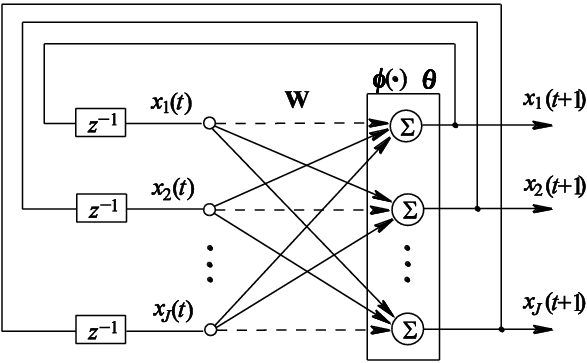
\includegraphics[width=0.3\textwidth]{hopfield.png}
\caption{Hopfield Model Neural Network}
\label{fig:tigre}
\end{figure}

\section{Desarrollo}

Antes de realizar el codigo para comprobar lo que vamos a realizar va a funcionar es necesario realizar un prototipado y para ello se hará uso de la heramienta octave, donde se realizará el prototipo de nuestra red neuronal hopfiel.\\
\\
Para comprender lo que se realizará la siguiente imagen muestra el ejemplo del funcionamiento de la red hopfiel en su comportamiento interno. 

\begin{figure}[htb]
\centering
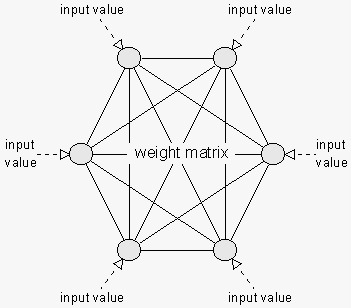
\includegraphics[width=0.5\textwidth]{hopfiel_startjpeg.jpeg}
\caption{Hopfield Model Neural Network Example}
\label{fig:tigre}
\end{figure}

Como se muestra en la imagen anterior lo que hará será comparar entre todos los valores de entrada y entregar el valor que mas se parece, para ello llamaremos a nuestros valores de entreada o valores de entrenamiento x1,x2,x3,x4...N, y realizaremos una sumatoria pondereada de dichos valores y los guardaremos en W, lo siguiente será hacer el calculo matematico e ir comparadado el patron mas parecido con el que deseamos como salida y deberá mostrarse por consola.
\\
\\
Durante el desarrollo de el codigo hubo algunos problemas que inpedian realizar el aprendizaje de la red neuronal y hacia que esta se confundiera con los calores que se le introducian para comparar con los de entranmiento, como primer inpedimento fue el tamaño de la matriz ya que antes planeaba realizar el abecedario japones con matices de 18 * 18, pero el tamaño era demasiado grande de las matrices , asi que fui incrementando poco a poco la matriz hasta obtener un buen resultado por parte de la red, durante la incrementación de las columnas y filas la red dejaba de funcionar por el segundo problema que fué el groso del simbolo a identificar, es decir, la representacion de 1's, ya que si era muy delgado la red se confundia y mostraba resultados erroneo, asi que probe engruesando el simbolo (letra coreana) y esta dió un buen resultado, sin embargo cabe mencionar que la posicion del simbolo en la matriz de 13 *13 tambien afectaba para el reconocimiento de patron, por ello decidi solo introducir 10 valores de entrenamiento para que funcionara correctamente y no se confundiera entre los simbolos o mostrara resultados no existentes.

La siguiente imagen muestra procesa los datos de entrada y salida de nuestro programa.


\begin{figure}[htb]
\centering
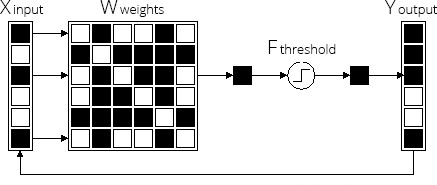
\includegraphics[width=0.8\textwidth]{hopfield-network.jpg}
\caption{Hopfield inner workings}
\label{fig:tigre}
\end{figure}

A continuación se muestran algunos de los datos de entrada que ocupé para hacer el entrenamiento de la red neuronal:
\\

\begin{figure}[htb]
\centering
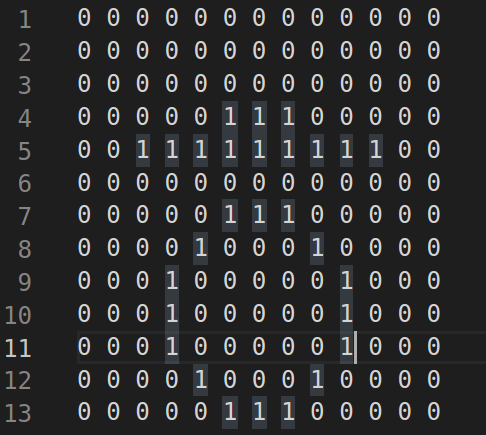
\includegraphics[width=0.6\textwidth]{letra_coreana_Ej1.png}
\caption{training example}
\label{fig:tigre}
\end{figure}

Y acontinuacion la siguiente imagen muestra los resultados de la red neuronal ya entrenada y comparando un valor que esperamos obtener, el resultado que se muestra es correcto sin embargo se puede apreciar al final de la matriz que no se alcanza a imprimir completamente.

\begin{figure}[htb]
\centering
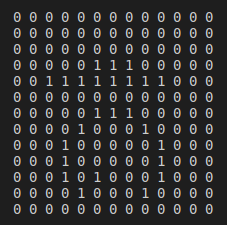
\includegraphics[width=0.6\textwidth]{code.png}
\caption{Results}
\label{fig:tigre}
\end{figure}




\section{Conclusión}
Mi conclusión es que el programa funciona correctamente sin embargo tiene algunas limitantes como es el tamaño de la matriz y la posición del la representación de la silueta, es decir, la colocación de los 1's dentro de la matriz, ya que tambien afecta a la hora de mostrar los resultados por la terminal, tambien los patrones de entrenamiento no deben ser iguales ya que estos ocasionan confusión en la red neuronal y provaca que imprima algunos patrones no existentes, por los problemas mencionados anteriormente fue que decidi elegir el tema de abecedario coreano y elegi las letras que no se parecian tanto para que fuera a la red mas facil identificar el patron que deaba obtener con los de entrenamiento.

	

\end{document}
